\section{Алгоритм построения фронта Парето}\label{sec:ch4/sec5}

В рамках разработанной методологии многокритериальной оптимизации параметров алгоритмов управления электропневматическим приводом реализован
метод NSGAII, основанный на принципах недоминируемой сортировки и концепции доминирования по Парето, описанной в уравнении \ref{eq:multiobjective_optimization}.

Принципиальной особенностью реализованного метода является совместное использование механизмов ранжирования на основе недоминируемой
сортировки и техники поддержания разнообразия решений с помощью опорных точек. Процесс оптимизации осуществляется следующим образом.

Начальное множество решений формируется путем случайной генерации векторов
параметров в заданных диапазонах допустимых значений. Для каждого 
вектора вычисляются значения целевых функций согласно улсовиям описанных в выражении \ref{eq:dominance}. 

Ключевым элементом метода является процедура быстрой недоминируемой сортировки, которая разделяет текущее множество решений
на фронты $F_1, F_2, ..., F_k$ в соответствии с отношением доминирования. Для каждого решения $p$ определяются два множества:

\begin{equation}
S_p = \{q \in P | p \prec q\} \quad \text{множество доминируемых решений}.
\end{equation}

\begin{equation}
n_p = |\{q \in P | q \prec p\}| \quad \text{количество доминирующих решений}.
\end{equation}
где $P$ -- текущее множество решений, символ $\prec$ обозначает отношение доминирования.

Решения с $n_p = 0$ формируют первый фронт $F_1$. Для каждого решения $p \in F_1$ просматриваются
все доминируемые им решения $q \in S_p$ и уменьшается их счетчик $n_q$ на единицу.
Решения, для которых $n_q$ становится равным нулю, формируют следующий
фронт $F_2$. Процесс продолжается до исчерпания всего множества.

На рисунке \ref{fig:pareto_sorting} показан пример недоминируемой сортировки для множества решений в двумерном пространстве целевых функций.

\begin{figure}[ht]
    \centering
    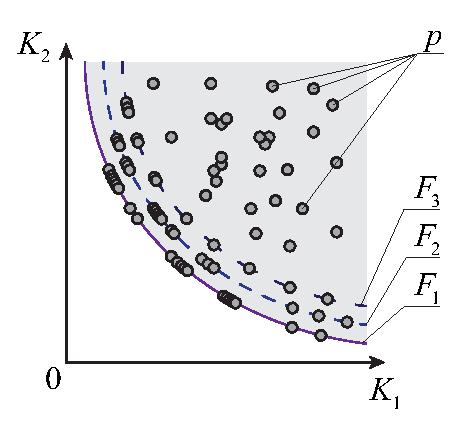
\includegraphics[]{part4/pareto_sorting.eps}
    \caption{Пример недоминируемой сортировки для множества решений в двумерном пространстве целевых функций}
    \label{fig:pareto_sorting}
\end{figure}

Итерационный процесс оптимизации реализуется с помощью модифицированных операторов:

\begin{enumerate}
\item Селекция методом турнирного отбора с учетом рангов доминирования, где вероятность выбора решения обратно пропорциональна номеру фронта, к которому оно принадлежит;

\item Оператор рекомбинации с имитацией бинарного скрещивания:

\begin{equation}
c_{1,2} = 0.5[(1 \pm \beta)p_1 + (1 \mp \beta)p_2]
\end{equation}
где параметр $\beta$ определяется через:
\begin{equation}
\beta = \begin{cases}
(2u)^{\frac{1}{\eta_c + 1}}, & \text{если } u \leq 0.5 \\
(\frac{1}{2(1-u)})^{\frac{1}{\eta_c + 1}}, & \text{иначе}
\end{cases}
\end{equation}
где $u$ -- случайное число из интервала $[0,1]$;
$\eta_c$ -- параметр распределения оператора рекомбинации;

\item Оператор мутации с полиномиальным распределением и адаптивной вероятностью:

\begin{equation}
c_m = c + \delta(u_b - l_b),
\end{equation}
где возмущение $\delta$ вычисляется как:

\begin{equation}
\delta = \begin{cases}
(2r)^{\frac{1}{\eta_m + 1}} - 1, & \text{если } r < 0.5 \\
1 - (2(1-r))^{\frac{1}{\eta_m + 1}}, & \text{иначе}
\end{cases}
\end{equation}

где $r$ -- случайное число из интервала $[0,1]$;
$\eta_m$ -- параметр распределения мутации;
$u_b$ и $l_b$ -- верхняя и нижняя границы параметра соответственно.
\end{enumerate}

Для сохранения разнообразия множества решений и равномерного распределения точек вдоль фронта Парето
применяется механизм ассоциации с опорными точками. Опорные
точки генерируются равномерно в нормализованном
пространстве целевых функций. Для каждого решения вычисляется расстояние до опорных точек:

\begin{equation}
d(\mathbf{f}, \mathbf{r}) = \|\mathbf{f}_n - \mathbf{r}\|,
\end{equation}
где $\mathbf{f}_n$ -- нормализованный вектор целевых функций:

\begin{equation}
\mathbf{f}_n = \frac{\mathbf{f} - \mathbf{f}_{min}}{\mathbf{f}_{max} - \mathbf{f}_{min}}.
\end{equation}

При формировании нового множества решений применяется элитарная стратегия, при которой сначала включаются полные
фронты, начиная с первого. Для последнего включаемого фронта используется механизм
кластеризации на основе ассоциации с опорными точками, что обеспечивает равномерное заполнение фронта Парето.

\subsection{Генерация начальной выборки методом латинского гиперкуба}\label{sec:ch4/sec4/subsec1}
Для обеспечения эффективного построения суррогатных моделей и последующего поиска
оптимальных параметров алгоритмов управления электропневматическим приводом существенное
значение имеет формирование начальной выборки в пространстве параметров.
Метод латинского гиперкуба (LHS) позволяет осуществить стратифицированную выборку
многомерных параметров с обеспечением равномерного покрытия области поиска.

Пусть пространство параметров алгоритма управления задано
вектором $\mathbf{x} \in \mathbb{R}^d$, где $d$ - размерность пространства параметров.
Для каждого параметра определен допустимый интервал значений:
\begin{equation}
x_i \in [a_i, b_i], \quad i = 1,\ldots,d
\end{equation}
где $a_i$ и $b_i$ -- нижняя и верхняя границы интервала для $i$-го параметра соответственно.

При формировании выборки объема $N$ методом латинского гиперкуба
осуществляется разбиение каждого интервала
на $N$ непересекающихся подинтервалов равной вероятности:
\begin{equation}
[a_i + \frac{k-1}{N}(b_i - a_i), a_i + \frac{k}{N}(b_i - a_i)], \quad k = 1,\ldots,N
\end{equation}
Генерация точек выборки производится согласно следующему алгоритму:

Формируется матрица $\mathbf{P} \in \mathbb{R}^{N \times d}$, где каждый столбец содержит случайную перестановку чисел от 1 до $N$.
Генерируется матрица случайных чисел $\mathbf{R} \in \mathbb{R}^{N \times d}$ с равномерным распределением на интервале $[0,1]$.
Вычисляются координаты точек выборки:

\begin{equation}
x_{ij} = a_i + \frac{p_{ij} - 1 + r_{ij}}{N}(b_i - a_i)
\end{equation}
где $x_{ij}$ -- значение $i$-го параметра для $j$-й точки выборки;
$p_{ij}$ -- элемент матрицы перестановок, $r_{ij}$ - элемент матрицы случайных чисел.

Для повышения равномерности покрытия пространства параметров применяется
оптимизация выборки путем минимизации критерия максимальной корреляции между столбцами:
\begin{equation}
\min_{\mathbf{P}} \max_{i,j} |\rho(x_i, x_j)|, \quad i \neq j
\end{equation}
где $\rho(x_i, x_j)$ -- коэффициент корреляции Пирсона между векторами значений $i$-го и $j$-го параметров.

Оптимизация осуществляется методом имитации отжига с целевой функцией:
\begin{equation}
f(\mathbf{P}) = \sum_{i=1}^{d-1}\sum_{j=i+1}^d |\rho(x_i, x_j)|^q
\end{equation}
где $q$ -- показатель степени, обычно принимаемый равным 2.

Полученная оптимизированная выборка обеспечивает равномерное покрытие пространства
параметров и минимальную корреляцию между параметрами, что способствует повышению
точности последующего построения суррогатной модели и эффективности поиска оптимальных параметров алгоритма управления.